\chapter{Specification}
The specification of the program defines \textbf{what it does} rather than how.
This chapter presents the specification of the system taking into consideration general software engineering principles, the models proposed by Larman  in \cite{Larman:2004} (at least conceptual, use case and behaviour models) and Meyer's (FIXME CITE??) \ac{DbC}.
For the particular case of this thesis, the specification takes into account reengineering principles and procedures and \ac{TDD} as a tool to define what the system does as opposed to a simple testing technique.

Reengineering software comprises 6 activities (\fref{sec:reengineering}): 
\begin{enumerate}
    \item Inventory Analysis
    \item Documentation Restructuring
    \item Reverse Engineering
    \item Code Restructuring
    \item Data Restructuring
    \item Forward Engineering
\end{enumerate}   
   
The outcome of these activities derives part of this specification.
For example, use cases are extracted from the current system.
The first three focus on what the system does and are used in this chapter, whereas the last three are tightly coupled to technology and are expanded in \fref{chap:design}.

This chapter starts by describing the \textbf{current system}: the software parts (\textbf{inventory analysis}) and what it does (\textbf{reverse engineering} to understand the system with special attention to \textbf{context}, \textbf{interaction} and \textbf{interoperability}).
It is followed by a description of what the \textbf{new system} has to do: the \textbf{specification} comprises a \textbf{conceptual model}, a \textbf{use case model} and a \textbf{behaviour model}.
FIXME Finally, it describes the \ac{XML} used to represent content applications.

\section{Inventory Analysis}
A list of software in the organisation makes candidates for reengineering appear.
The scope of this thesis is reengineering Flango \cm in the robot and it is a decision taken before starting this work.
\begin{inventory}
{name=Flango \cm (robot),
lbl=inventory-flango-cm, 
year=May 2011,
nchanges=5 big milestones,
lastchange=August 2013,
sysresides=Reem H2 and H3,
appinterfaces=Flango Backend; robotBehaviour,
dbs=SQLite in the robot (exclusive use),
projLongevity=Until September 2013,
projNchanges36=0,
maintenCost=1 software engineer full-time
}
\end{inventory}

\begin{inventory}
{
name=\flangofe -- \se , 
lbl=inventory-flango-se, 
year=December 2012,
nchanges=4 (first version; some new features; bug fixing),
lastchange=August 2013,
sysresides=Basestation,
appinterfaces=Flango Frontend (robot); Flango Backend,
dbs=flango (postgresql through the Backend),
projLongevity=At least until January 2015,
projNchanges36=Bug fixing,
maintenCost=1 software engineer full-time
}
\end{inventory}

\begin{inventory}
{
name=\flangobe , 
lbl=inventory-flango-be, 
year=October 2012,
nchanges=3 (first version; statistics; new features),
lastchange=August 2013,
sysresides=Basestation,
appinterfaces=Flango Frontend (robot); Flango Screens Editor,
dbs=flango (postgresql),
projLongevity=At least until January 2015,
projNchanges36=Unspecified number of new features and bug fixing,
maintenCost=1 software engineer full-time
}
\end{inventory} 

However, Flango \cm uses other software (\ref{inventory-flango-se} and \ref{inventory-flango-be} ) that might have to be reengineered in the future or even modified to suit the needs of the new technology in the project.

When it was decided to reengineer \flangofe it was not very old but there were major changes already contemplated for the application (e.g. abandon \flash), that would require big commitment of effort and that would not converge to a sustainable situation.
Reengineering costs are lower than the cost to make changes plus the cost of maintenance.

\section{Reverse Engineering}
\label{sec:reverse-eng}
Reengineering a software involves reverse engineering, \textbf{understanding what the system does}.

There are 3 key issues in understanding the current system: \textbf{abstraction level}, \textbf{completeness} and \textbf{direction}.
This specification uses a system-level abstraction, only takes into account interaction with external elements, and is one-way (from current system to the specification of the new system).
Other levels of abstraction do not apply here to keep this specification technology-agnostic.
This section focuses on what the current version of the software does and what the new version has to do.
It offers some technology-dependant details to understand the steps to reach the goal and the operations that Basestation exposes.

Details of how this software does the same with a new technology are in \fref{chap:design} and \fref{chap:implementation}

\subsection{Context}
\label{sec:context}

\begin{figure}[htb]
    \centering
    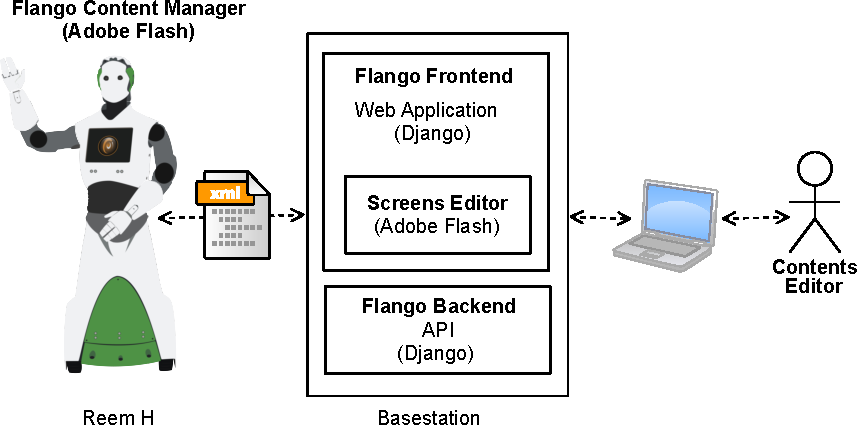
\includegraphics{figures/context-original.pdf}
    \caption{Reverse engineering: Current context}
    \label{fig:context-original}
\end{figure}

\begin{figure}[htb]
    \centering
    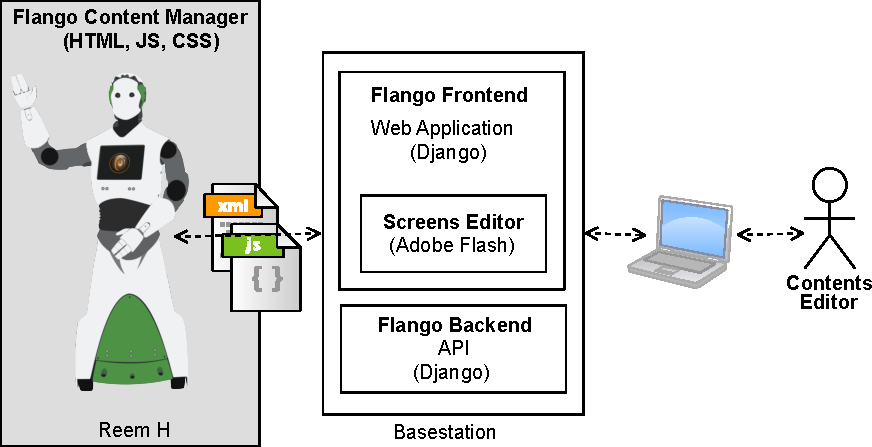
\includegraphics{figures/context-new.pdf}
    \caption{Reverse engineering: New context}
    \label{fig:context-new}
\end{figure}

\reem{H3} has about 600MB of specialised code.
The program that glues all software parts and serves as an interface to the hardware is \textbf{robotBehaviour}, developed with Qt.
A window in this program contains a QtWebKit widget, the embedded web browser that loads the contents for the touchscreen.
Contents are fetched from Basestation, a server that hosts Flango, a web application that lets users edit screens (with the \se), add media contents and synchronise them with robots (\ref{fig:context-original} on \pageref{fig:context-original}).
The \flangobe has an \ac{API} to serve the content applications to the robots.
The project of this thesis is reengineering the Flango \cm , in the robot (\fref{fig:context-new}).

\FloatBarrier

\subsection{Interaction} 
\label{sec:interaction}
\begin{figure}[htb]
   \centering
   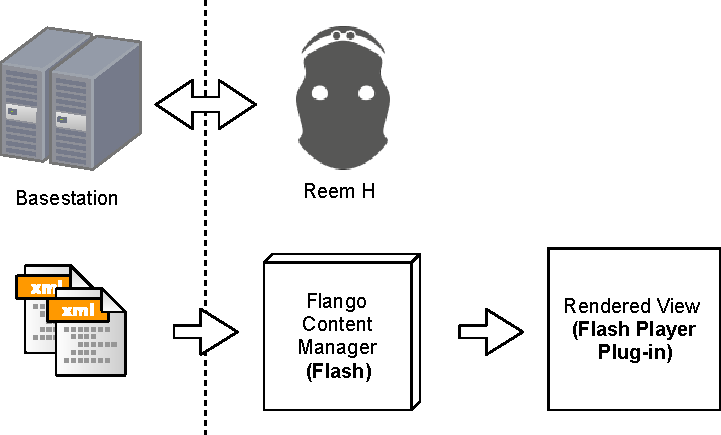
\includegraphics{figures/interaction-original.pdf}
   \caption{Reverse engineering: Current interaction}
    \label{fig:interaction-original}
\end{figure}

\begin{figure}[htb]
    \centering
    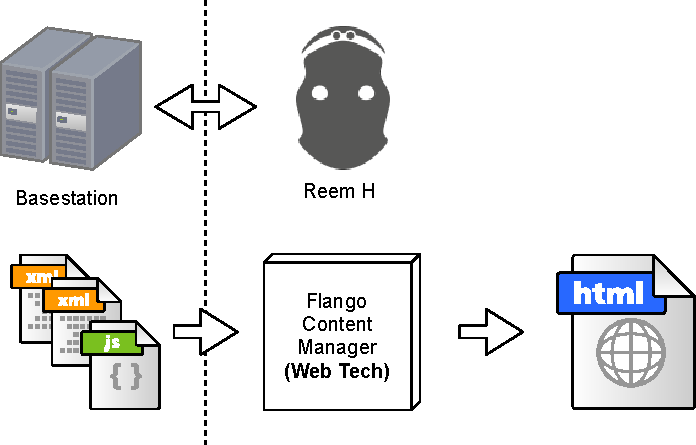
\includegraphics{figures/interaction-new.pdf}
    \caption{Reverse engineering: New interaction}
    \label{fig:interaction-new}
\end{figure}

The \cm 's input is \ac{XML} code and the output is an \ac{HTML} single page application (\fref{fig:interaction-original} and \fref{fig:interaction-new}).
The general boot sequence is:

\begin{enumerate}
    \item The robot boots
    \item robotBehaviour fetches generic settings (\ac{XML}) from Basestation
    \item The \cm uses the settings to decide which application to load, the language, the theme, etc. It requests application-specific settings and the application structure. After this, it requests the screens (the \ac{XML} files) to the \flangobe .
    \item Basestation serves all the screens
    \item The \cm renders the screens. If during this process it finds an "entity", it fetches the data from Basestation.
\end{enumerate}

\FloatBarrier

\subsection{Interoperability}
\label{sec:interoperability}
\begin{figure}[htb]
  \begin{minipage}{0.5\linewidth} 
      \centering
      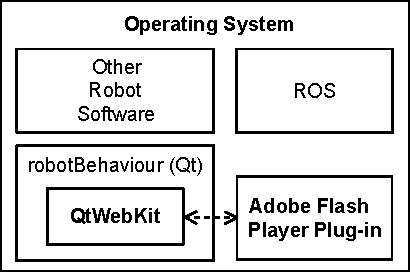
\includegraphics{figures/interoperability-original.pdf}
      \caption{Reverse engineering: Current interoperability \\ (in robot)}
      \label{fig:interoperability-original}
  \end{minipage}
  \hspace{0.5cm}
  \begin{minipage}{0.5\linewidth} 
      \centering
      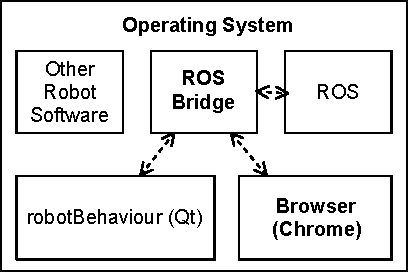
\includegraphics{figures/interoperability-new.pdf}
      \caption{Reverse engineering: New interoperability \\ (in robot)}
      \label{fig:interoperability-new}
  \end{minipage}
\end{figure}

Flango \cm interoperates with two systems: robotBehaviour and \flangobe (See figures \ref{fig:interoperability-original} and \ref{fig:interoperability-new} on \pageref{fig:interoperability-original}).

\paragraph{robotBehaviour} Flango \cm interoperates with the software of the robot through robotBehaviour, e.g. using text-to-speech capabilities or triggering a batch action (autopresentation, guide user to a certain place...).
Likewise, robotBehaviour uses an \ac{API} in Flango \cm , e.g. to restart a session or to display a screen.
There is an interface defined for this to allow independent development in both ends.

The current system to exchange messages between the \flash container and robotBehaviour is based on JavaScript global functions.

To send a message to robotBehaviour:
\begin{enumerate}
    \item \cm (\flash) opens a new tab with a specific \ac{URL}: \texttt{flashCallback.html?\textless paramList\textgreater}
    \item robotBehaviour intercepts the call, prevents QtWebKit from opening a new tab and executes an action specified with the parameters
\end{enumerate}

To send a message from robotBehaviour:
\begin{enumerate}
    \item Calls a \ac{JS} function in the Flash website (\texttt{/static/frontend/index.html})
    \item The \ac{JS} function delegates to the Flash container
    \item The application facade of Flango Content Manager starts the required action
\end{enumerate}

The requirements state that the new software has to be implemented using web technology. 
Despite the fact that this specification should be technology agnostic, to integrate the new software better in the system, the use of \ac{ROS} Web Tools is suggested to exchange messages.
In any case, it is clear that there has to be an interface between robotBehaviour and the browser, as they run in separate processes (as opposed to sharing at least one parent process in the current implementation).

\paragraph{BaseStation (\flangobe \ac{API})} The \cm has to fetch data from Basestation in order to load the correct contents.
The \flangobe has an \ac{API} for this (\fref{tab:flango-api}):

\begin{table}[ht]
    \centering
    \begin{tabularx}{\linewidth}{| l | X |}
    \hline
    Root URL & Matching URLs \\
    \hline
    \multirow{2}{*}{\texttt{flango-api-0.1/robots}}
        & get\_robots \\ 
        & add\_robot \\
    \hline 
    
    \multirow{2}{*}{\texttt{flango-api-0.1/bl}} 
        & entity/(\textless entity\_name\textgreater).xml \\ 
        & add\_robot \\
    \hline
    
    \multirow{6}{*}{\texttt{flango-api-0.1/pal}} 
        & home \\
        & add \\
        & execute \\
        & status \\   
        & submit \\
        & history/(\textless page\textgreater) \\
    \hline
    
    \multirow{10}{2.5cm}{\texttt{flango-api-0.1/gui}  \texttt{flango-api-0.1/app}}
        & \textless app\_id\textgreater /config.\textless format\textgreater xml$|$json \\
        & \textless app\_id\textgreater /structure.\textless format\textgreater xml$|$json \\
        & \textless app\_id\textgreater /screen/(\textless screen\_id\textgreater.xml \\
        & \textless app\_id\textgreater /node/\textless node\_id\textgreater \\
        & application \\
        & node \\
        & screen \\
        & allScreens \\
        & getApps \\
        & upload\_app \\
    \hline
    
    \multirow{7}{*}{\texttt{flango-api-0.1/stats}}
        & robot/use/\textless robotID>/\textless duration\textgreater/<data\textgreater \\
        & robot/base \\
        & app/use/\textless robotID\textgreater/\textless duration\textgreater/<data\textgreater \\
        & app/top/\textless robotID\textgreater/\textless duration\textgreater/<data\textgreater \\
        & app/toptable/\textless page\textgreater \\
        & application/\textless screen\textgreater \\
        & \textless name\textgreater \\
    \hline
    \end{tabularx}
    \caption{Flango Backend \ac{API}}
    \label{tab:flango-api}
\end{table}
Both current and new implementation use this.
However, the new implementation uses \ac{JSON} because it is more \ac{JS}-friendly: it has less overhead and it is easier to deserialise.

\section{Conceptual Model}
\begin{sidewaysfigure}[htb]   
    \centering
    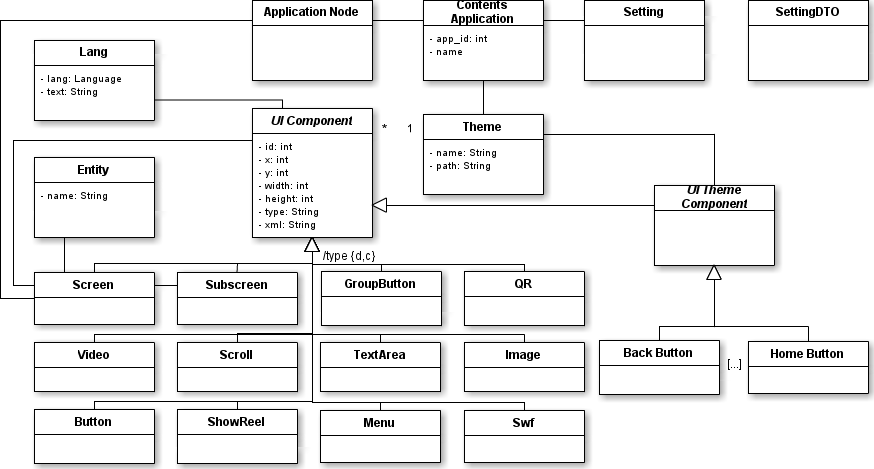
\includegraphics[width=\textwidth]{figures/specification-conceptual-model}
    \caption{Conceptual model}
    \label{fig:specification-conceptual-model}
\end{sidewaysfigure}

The new Flango \cm has to be compatible with the current implementation of the \se (\flangofe).
Otherwise, users would create content applications with the \se that would look different when they are displayed in the robot.
To ensure compatibility, it is necessary a good understanding not only at system level, but at component level.
It is required, then, that the new implementation displays consistently all of the \ac{UI} components that the \se can create exactly like it does with the old version. 
Same applies to settings and use of entities.

There are 7 classes: \textbf{ContentsApplication}, \textbf{ApplicationNode}, \textbf{Configuration}, \textbf{Theme}, \textbf{Screen}, \textbf{UI Components} and \textbf{Entity}.

\begin{description}
\item[ContentsApplication] A contents application with an internal identifier and a descriptive, human-friendly name.
\item[ApplicationNode] An application has nodes that match the \ac{URI} with a screen.
\item[Configuration] A contents application has a configuration object that can be mutated during the execution.
It represents the state of the application, the permissions, paths, etc.
\item[Theme] Themes are the look and feel and default behaviour of \ac{UI} components.
The current implementation only has one (default) theme.
However, a contents application can have many themes available.
The active theme has to belong to the set of available themes. 
It encapsulates data that define it (e.g. the name, etc).
\item[Screen] The container for UI Components.
\item[UI Components] A UI Component is an element of the \ac{UI}, for example a \texttt{Button} or an \texttt{Image}, that has an \ac{XML} code associated.
Users drag and drop them to a canvas in the \se to create the contents. 
Because the domain of the problem and the classes are shared between the original and the new implementation, the model in \fref{fig:specification-conceptual-model} is created from the current implementation.
To support themes, there are two types of UI Components: basic (UI Component) and theme (UI Theme Component).
All UI Theme Components are eventually implemented with a basic UI Component.
\end{description}

Listings \ref{uicomponents-list} and \ref{uithemecomponents-list} in \fref{chap:app-uicomponents} contain a comprehensive list of UI Components extracted from listing the necessary files in a package of the current implementation.
All files in \ref{uicomponents-list} have the corresponding class in the conceptual model if they have to be implemented.
The elements of \ref{uithemecomponents-list} are in fact folders but they can be considered classes in this specification as they are part of the domain of the problem.
However, some elements are not to be implemented because they are deprecated and some other components are to be implemented in future releases, but not in the software of this thesis.

\subparagraph{Excluded elements} UI Components: GroupButtonComponent, GroupComponent, ScrollComponent. UI Theme Components: call\_to\_action\_screen, main\_menu, smartphone\_menu, synchronizing\_screen.

\paragraph{Configuration} The state of the application is defined with a configuration object sent from the server.
A collection of the necessary attributes of the class that encapsulates the configuration is in \ref{uithemecomponents-list} and has been extracted from the current implementation as well.
\subparagraph{Excluded elements} Some Configuration have names tightly coupled to technology (e.g. history, history\_current, etc). 
The concept is included in the specification but not with this specific names to keep it technology agnostic.

\paragraph{Entity} Entities are classes that represent classes in the \se . 
An example scenario: Alice is creating screens with the \se .
She rented the robot for a congress and wants to add information about job openings in her company.
She can define, with \flangofe , an entity named "Job" and use it in the screens editor to show the list of all instances of Job.
The implementation of Entities is incomplete and does not belong to the scope of this project.

\paragraph{Themes} A Contents Application can have themes.
There is a default theme that defines the look and feel and default actions on click an on load of all UI Theme Components.
All themes have the same UI Theme Components to guarantee that themes can be changed safely.
Basic UI Components look always the same way.

Listing \ref{design-specification-button-example-1} shows an example of the \ac{XML} definition of a Button UI Component.

\lstinputlisting[label=design-specification-button-example-1, language=XML, caption={Basic UI Component Button XML}]{src/specification-button-example-1.xml}

\FloatBarrier

\section{Use Case Model}
This section describes the services of the system as sequences of events triggered by external actors.

\subsection*{Actors}
The actors who use the system are:
\begin{description}
	\item[robotBehaviour] The software that governs the \ac{GUI} of the touchscreen. It can load content applications, bring them to the front, sent them to the back, load other \acp{GUI} etc.
	\item[Contents Application User] A person (or any other agent that can use a touchscreen) who interacts with the loaded contents application. Humans only interact directly with the output of this software (see \fref{sec:context}), which becomes the \ac{GUI}.
For example: the program displays a screen with one button whose action is to make Reem say "hi, my name is Reem".
The input is an \ac{XML} file, the output is a \ac{GUI} ready to be used.
Humans can now touch the button that sends events to robotBehaviour so, essentially, the \ac{GUI} of the program and not only the output is built as a function of the input.
When the \ac{GUI} is ready, a new actor (Contents Application User) and new use cases appear.
\end{description}

\subsection*{System Use Cases}
\begin{figure}[htb]  
    \centering
    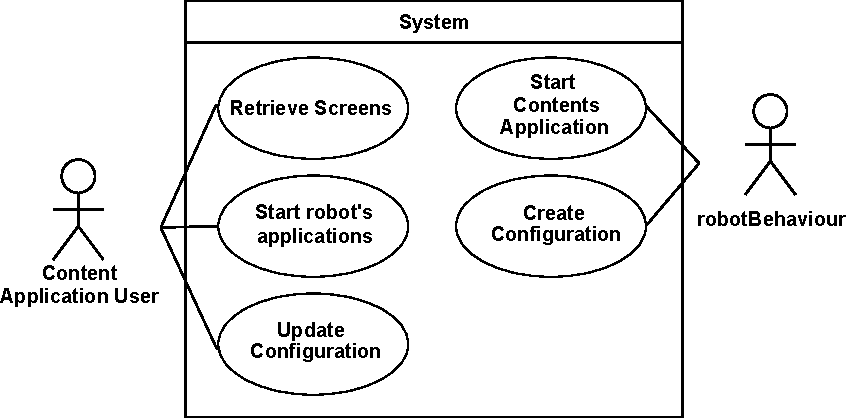
\includegraphics[width=\linewidth]{figures/specification-sucs}
    \caption{System Use Cases}
    \label{fig:specification-sucs}
\end{figure}

There is a number of use cases of the software determined by examining the current implementation at a program level.
The use cases that are implemented in this project are shown in \fref{fig:specification-sucs}.

A contents application user can see the rendered screens and update some parameters (e.g. change the language) or start applications in the robot (e.g. a Qt window with a map).
The software system that controls the robot, robotBehaviour, can also trigger actions in the contents application (for example, it can start it).
Amongst others, it can manage some special settings (including: show the cursor, enable debug mode, etc). 

\begin{suc}
{Start Robot's Applications}
{A user can start robot's applications like face recognition, ball grasping, meet people, etc.}
{Content Application User}
{robotBehaviour is running}
{The chosen robot application starts}
{
    \begin{enumerate}
        \item The User chooses a robot's application and asks the system to start it
        \item The system starts the application
    \end{enumerate}
}
{None}
\end{suc}

\begin{suc}
{Start contents application}
{robotBehaviour wants to display the application on the touchscreen of the robot}
{robotBehaviour}
{
	\begin{enumerate}
        \item robotBehaviour is running
        \item The application has been synchronised with the robot (i.e. the robot has all the necessary parts to load it)
    \end{enumerate}
}
{
The initial screen of the contents application is shown
}
{
    \begin{enumerate}
        \item robotBehaviour determines the $app_id$ and asks the system to load the application with the given $app_id$ and initialisation parameters.
        \item include Manage Configuration
		\item the system loads the initial screen
    \end{enumerate}
}
{    
	\begin{itemize}
        \item The application can not be found
        \begin{enumerate}
        	\item The system shows a default screen
    	\end{enumerate}
    	\item The application contains errors
        \begin{enumerate}
        	\item The system degrades progressively the contents application
    	\end{enumerate}
    \end{itemize}    
}
\end{suc}


\begin{suc}
{Manage Configuration -- Create}
{The system fetches the configuration (on load) from the Backend. If it can not be found, it falls back to a default configuration. FIXME: no clear actor}
{Event on-load}
{
	\begin{enumerate}
        \item robotBehaviour is running
        \item The application has been synchronised with the robot
    \end{enumerate}}
{
The configuration object is created\footnote{Delete and read configuration are internal operations}
}
{
    \begin{enumerate}
        \item robotBehaviour starts the Flango Content Manager
        \item The system requests the generic configuration to the Backend
		\item The Backend sends the generic configuration $c$
		\item The system requests the application-specific configuration for application $c.app_id$ or $auto$
		\item The Backend returns the application-specific configuration $sc$
		\item The system requests the application structure
		\item The Backend returns the application structure $as$
		\item The system reads the URL query string that overwrites parameters
		\item The system creates the configuration object
    \end{enumerate}
}
{    
	\begin{itemize}
        \item The generic configuration can not be found
        \begin{enumerate}
        	\item The system displays an error message
    	\end{enumerate}
    	\item The application specific configuration can not be found
        \begin{enumerate}
        	\item The system loads the default application and displays an error message
    	\end{enumerate}
    	\item The application structure can not be found
        \begin{enumerate}
        	\item The system displays an error message
    	\end{enumerate}
    \end{itemize}   
}
\end{suc}

\begin{suc}
{Manage Configuration -- Update}
{The contents application user changes a parameter in the configuration or an event related to update the configuration is received}
{Contents Application User, events}
{
	\begin{enumerate}
        \item robotBehaviour is running
        \item The application has been synchronised with the robot
        \item The configuration object is initalized
    \end{enumerate}
}
{
The configuration object is mutated
}
{
    \begin{enumerate}
        \item The user asks the system to retrieve the configuration object
        \item The system returns the configuration object
        \item The user changes a value and asks the system to store it (e.g. current language)
		\item The system updates the configuration object (FIXME and notifies the system?)
    \end{enumerate}
}
{     
}
\end{suc}


\begin{suc}
{Retrieve Screen}
{The content application user navigates to a screen }
{Contents Application User}
{
	\begin{enumerate}
        \item robotBehaviour is running
        \item The application has been synchronised with the robot
        \item The application is loaded
    \end{enumerate}
}
{
The requested screen is shown
}
{
    \begin{enumerate}
		\item The user asks the system a list of screens (e.g. a screen with buttons)
        \item The system offers a list of screens to go
        \item The user chooses a destination
        \item The system shows the requested screen
    \end{enumerate}
}
{
    \begin{itemize}
	    \item The screen is unavailable
	    \begin{enumerate}
	    	\item The system shows an error
	    \end{enumerate}
    \end{itemize}
		
}
\end{suc}

\FloatBarrier

\section{Behaviour Model}
This thesis combines \ac{DbC} and \ac{TDD}, two techniques that are not mutually exclusive.
Basically, \textbf{tests define the behaviour for specific cases and \ac{DbC} defines the general behaviour}. 
Thus, there are no tests for edge cases or negative behaviours because contracts, and more specifically preconditions, protect the component.
In spite of the name, \ac{TDD} tests are executable specifications.
They become tests only after having implemented all the functionality being test-driven.
Before this, there is nothing to actually test and these artifacts are rather executable specifications, but not tests.
\textbf{Tests (specifications) are written before the code and define the behaviour of component}s.

Additionally, they are used as documentation of the software but they are not sufficient to completely define the behaviour because they only assert properties by example instead of stating general properties (e.g. "it should return 5" vs "return value $1 \leq x \leq 10$"). The latter can be described with formal specifications, e.g. using Meyer's \ac{DbC} \cite{Baumeister:2004}.

In this thesis, tests are implemented with Jasmine and AngularJS but this chapter focuses on what the tests describe rather than how they are executed and controlled.

Combining the two techniques one can use the best parts of each to define the behaviour of the system.
With \ac{TDD}:
\begin{itemize}
    \item Build only what is required (Keep it simple and control the scope of the project)
    \item Drive design decisions from tests (i.e. from the specification)
\end{itemize}

\noindent With formal specifications (\ac{DbC}):
\begin{itemize}
    \item Higher code quality
    \item Less checks (preconditions)
    \item Drive design decisions from preconditions
\end{itemize}


\textbf{Contracts of operations} define system behaviour and describe the outcome of executing system operations in terms of state changes to domain objects.
This section contains the sequence diagrams and contracts of the most relevant operations in the system.
However, the most complex part of this project is parsing and rendering the input \ac{XML} files.
Users do not interact directly with them: they do not execute operations that result in state changes to the domain object.
\Fref{chap:design} explains this problem and the solution in detail.

\subsection{Sequence diagrams}
\begin{figure}[htb]
    \centering
    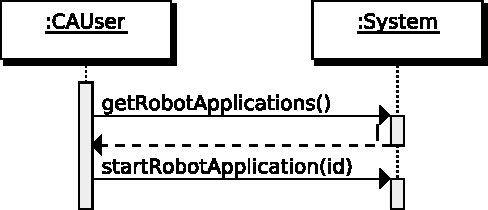
\includegraphics{figures/spec-seq-start-qtapp.pdf}
    \caption{System Sequence Diagram - Start Robot Applications}
    \label{fig:spec-start-qtapp}
\end{figure}

\begin{figure}[htb]
    \centering
    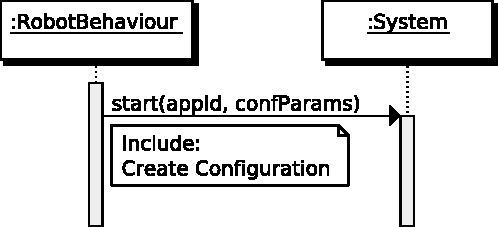
\includegraphics{figures/spec-seq-start-contents-app.pdf}
    \caption{System Sequence Diagram - Start Content Applications}
    \label{fig:spec-start-ca}
\end{figure}

\begin{figure}[htb]
    \centering
    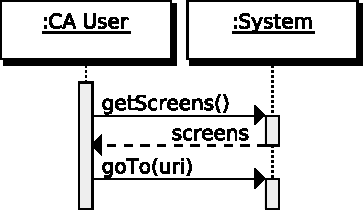
\includegraphics{figures/spec-seq-manage-screens-read.pdf}
    \caption{System Sequence Diagram - Manage Screens (Read)}
    \label{fig:spec-manage-screens-read}
\end{figure}

\begin{figure}[htb]
    \centering
    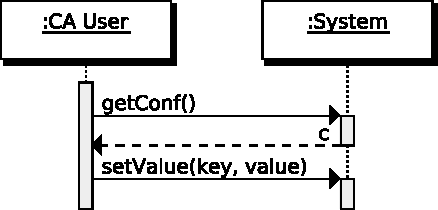
\includegraphics{figures/spec-seq-manage-conf-update.pdf}
    \caption{System Sequence Diagram - Manage Configuration (Update)}
    \label{fig:spec-manage-conf-update}
\end{figure}

\begin{figure}[htb]
    \centering
    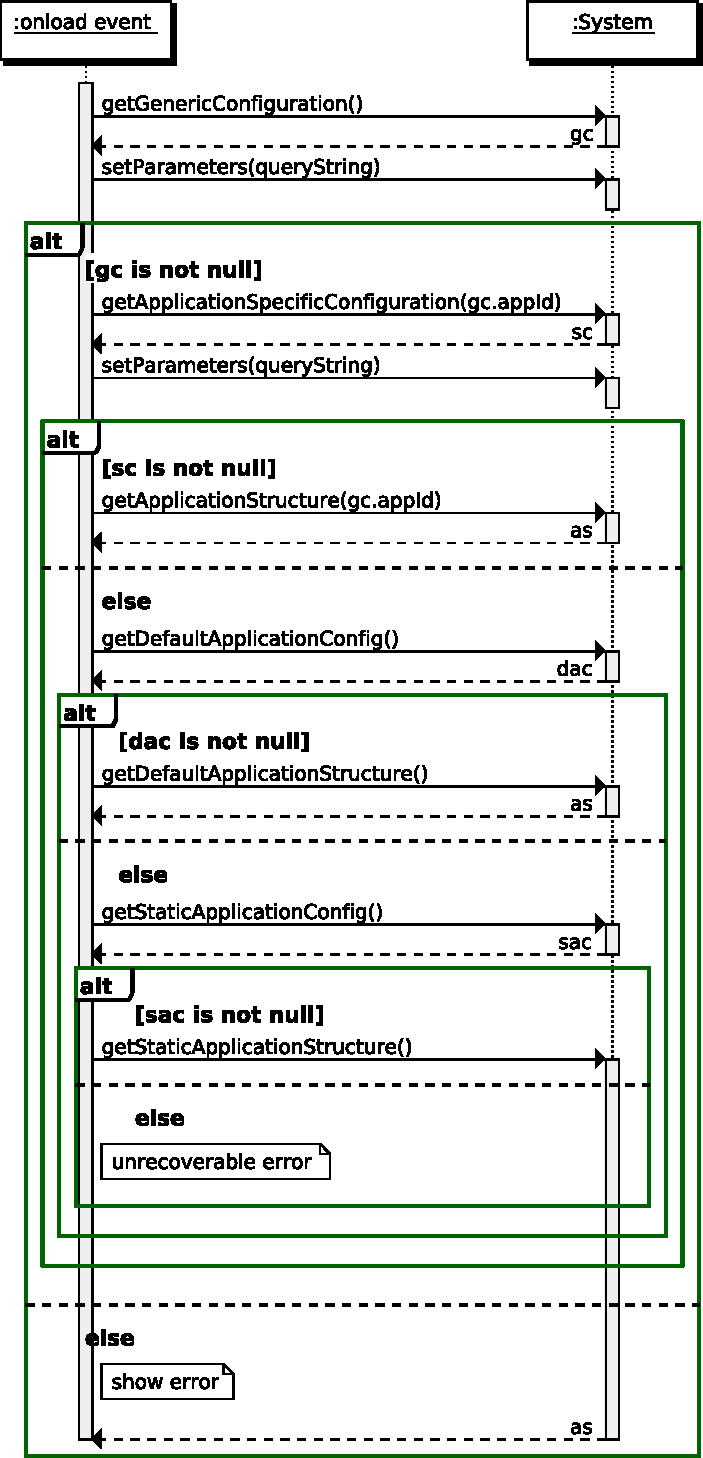
\includegraphics{figures/spec-seq-manage-conf-create.pdf}
    \caption{System Sequence Diagram - Manage Configuration (Create)}
    \label{fig:spec-manage-conf-create}
\end{figure}

\subsection{Contracts}

FIXME: robot behaviour ja no cal!!

\begin{sopcontract}{getRobotApplications()}
{FIXME: this is part of the contents of an XML file, like functions.xml. Maybe it should not be here. Retrieves a list of applications that can be launched from the Flango \cm , e.g. Qt applications like navigation or face recognition.}
{RobotBehaviour is running}
{A list \texttt{l} of robot applications was returned}
\end{sopcontract}

\begin{sopcontract}{startRobotApplication(id:String)}
{Starts the robot application with id \texttt{id}, e.g. 'face recognition'}
{\texttt{id} is a valid robot application identifier}
{A request to start the robot application with id \texttt{id} was sent}
\end{sopcontract}

\begin{sopcontract}{start(appId: Integer, confParams: HashMap)}
{Starts the contents  application with id \texttt{appId} and configuration parameters \texttt{confParam} that can overwrite the fetched configuration from the backend}
{\texttt{id} is a well-formatted contents application identifier}
{FIXME aaaa}
\end{sopcontract}

\begin{sopcontract}{getScreens(appId: Integer)}
{Obtains the screens of the contents application with id = \texttt{appId}}
{\texttt{id} is a well-formatted contents application identifier}
{A list of all screens of content applications with id = \texttt{appId} was returned}
\end{sopcontract}

\begin{sopcontract}{goTo(appId: Integer, uri: String)}
{Displays the desired screen}
{
\begin{enumerate}
    \item \texttt{id} is a well-formatted contents application identifier 
    \item \texttt{uri} is a well-formatted screen \ac{URI} in the contents application
\end{enumerate}
}
{\texttt{Conf.currentScreen} was set to \texttt{uri}}
\end{sopcontract}

\begin{sopcontract}{getConf(appId: Integer)}
{Obtains the local configuration object for the application \texttt{appId}. This object is stable during the execution of the program. It does not need to be fetched again from the Backend.}
{\texttt{id} is a well-formatted contents application identifier}
{The configuration \texttt{c} was returned}
\end{sopcontract}

\begin{sopcontract}{setValue(c: Conf, key, value)}
{Sets a field of the configuration object to the desired value.\\ e.g. \lstinline$setValue(c, 'currentLang', 'de')$}
{
\begin{enumerate}
    \item \texttt{key} is a valid field of the configuration object \texttt{c}
    \item \texttt{value} is a valid value for \lstinline$c[key]$
\end{enumerate}
}
{\lstinline$c[key]$ was set to \texttt{value}}
\end{sopcontract}

\subsection{Unit Tests}
The conceptual model in \fref{fig:specification-conceptual-model} describes the real world and shows the relationship between elements that define the problem.
Actors do not interact with most of the classes shown and contracts and sequence diagrams are intended to describe the system as a unit that provides some service to actors.
One of the goals of this project is making it compatible with the current \ac{XML} that defines the content applications.
To meet this goal, it should be clearly specified how \ac{XML} are parsed.
This project uses \ac{TDD} and has executable specifications for all parts of the system, including those (e.g. internal operations or parsing) that are not strictly eligible for other sections in this chapter.
Formally, an executable, technology-agnostic, specification might be written in \ac{OCL} and run in a \ac{UML} model.
These tests focus on the implementation and are written in JavaScript.
Even though they depend on technology, they define the system's behaviour and are considered part of the specification in this document.

Tests are organised in test-suites for components and each suite has several test cases.
This section focuses on the \ac{XML} description.

\Fref{chap:testing} has a full list and examples of other test suites that refer directly to components of the software (described in \fref{chap:design})
Tests challenge behaviour like reading text nodes in \ac{XML} tags, setting properties (i.e. mutating correctly an object in the system), reading order or inheritance of properties, fallback to default values and transformation to \ac{HTML} code.

An example of specifications by example of the UI directive:
\begin{enumerate}
	\item inline type property: should have type defined
	\item width, height, x, y, 
		\begin{enumerate}
			\item should set the property to 42 for the default (language-independent)
			\item should set the property to 40 for Catalan and 42 for French
			\item should set the property to 40 for Catalan, 42 for French and 20 for default
			\item should not set any property
			\item (inline) should set the property to 42 for the default (language-independent)
		\end{enumerate}
\end{enumerate}

\textbf{A comprehensive list is available in \fref{chap:app-unittests}}.

\section{XML Representation}
FIXME explain syntax here?

at least the inheritance and themes. with code.
